\documentclass[a4paper, british]{article}

\usepackage[utf8]{inputenc}
\usepackage[T1]{fontenc}
\usepackage{babel}
% \usepackage[margin=2.5cm,a4paper]{geometry}
% \usepackage[skip=1em]{parskip}
\usepackage{lmodern} 
\usepackage{microtype}
% \usepackage{xcolor}
\usepackage{graphicx}
\graphicspath{ {./figures/} }
% \usepackage{float}
% \usepackage{enumitem}
\usepackage{adjustbox} % rescale - useful for Dia exported TeX
\usepackage{tikz}
% \usepackage{pgfplots}
\usepackage{booktabs} %tables no vertical lines
% \usepackage{array}
% \usepackage{authblk}
% \usepackage{fancyhdr} %headers and footers
% \usepackage{titlesec}
% \usepackage{tcolorbox} % framed text boxes
% \usepackage{mathtools, amssymb, amsthm}
% \usepackage{gensymb}
\usepackage{chemformula} % chemical formulae
\usepackage{chemfig} % molecular figures
\usepackage{siunitx}
\usepackage{csquotes}
\usepackage[titletoc, title]{appendix}
% \usepackage{lettrine} % initials

\usepackage[
pdfauthor={Adam Menne},
pdftitle={Chemistry 264 - Practical 1},
pdfsubject={},
pdfkeywords={}]{hyperref}

\usepackage[noabbrev]{cleveref}

\usepackage[
backend=biber,
style=numeric,
sorting=none,
doi=true,
isbn=false
]{biblatex}
\addbibresource{citations.bib}

\setlength{\parskip}{1em}
\setlength{\parindent}{0em}
\linespread{1.3}

\title{Chemistry 264\\ Practical 1}
\date{Last editted on \today}
\author{Adam Menne\\ Stellenbosch University}

\begin{document}

\maketitle

\begin{abstract}
\noindent
In this practical a sodium hydroxide solution is standardised by titration with oxalic acid. Phenolphthalein was used as an indicator.
\end{abstract}

\tableofcontents

\newpage

\section{Introduction}

In this practical we carry out a series of acid-base titrations in order to standardise a sodium hydroxide solution. First an oxalic acid solution was prepared with a known concentration, which was then used to titrate the sodium hydroxide solution. Phenolphthalein was used as an indicator, to identify the equivalence point of the titrations. 

% \begin{figure}[htb]
%     \centering
%     \chemfig{
%         HO% 3
% -[:330,,2]% 1
%            (
%      =[:270]O% 4
%            )
%   -[:30]% 2
%            (
%       =[:90]O% 6
%            )
% -[:330,,,1]OH% 5
% }
% \end{figure}

\section{Results}

We find that our titrations were relatively consistent, \cref{fig:mean} shows the concentration of NaOH, calculated over five titrations. These values have a relative standad deviation of 1.569 as can be seen in \cref{table:data}, which also shows the mean and CI values.

\begin{figure}[h]
    \centering
    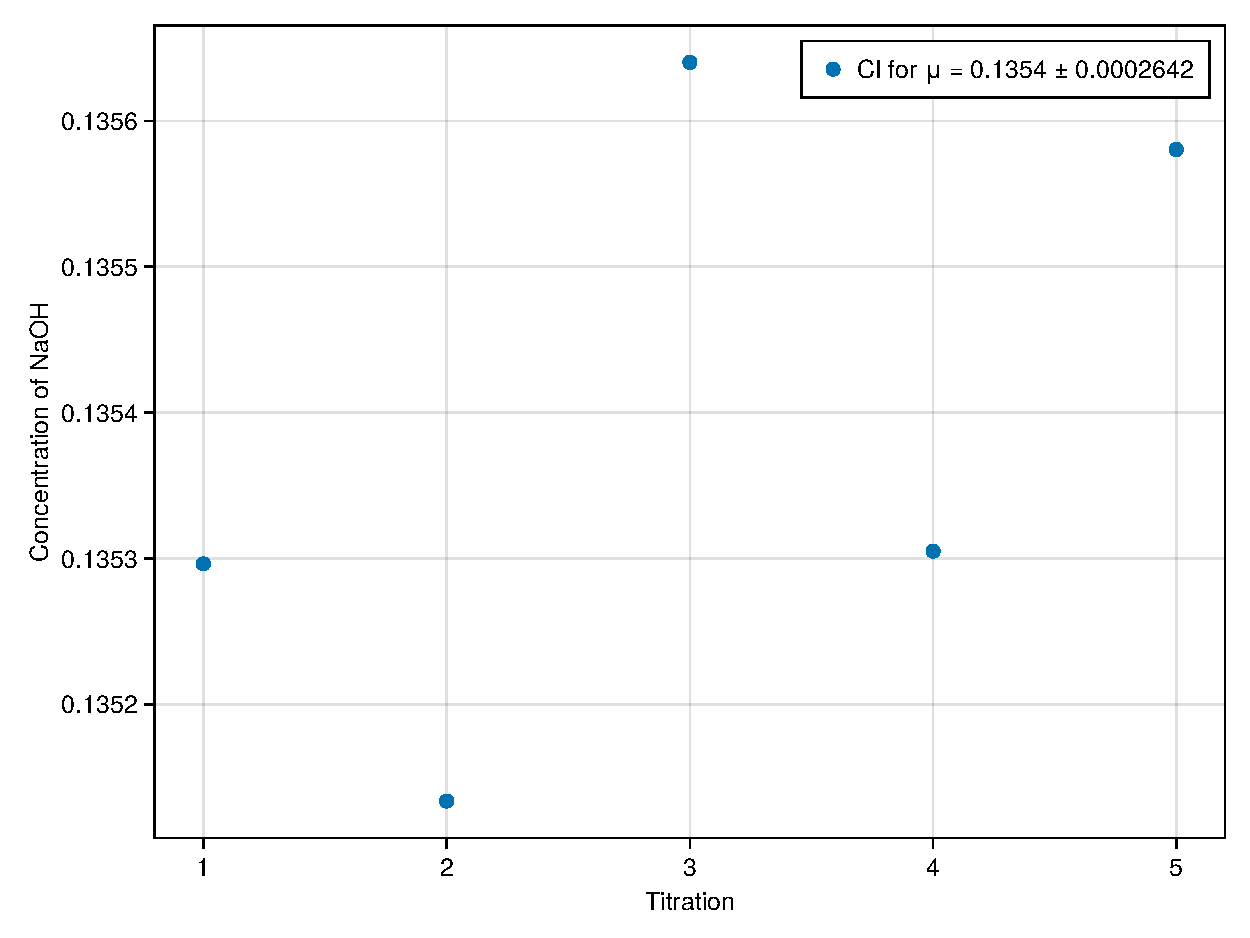
\includegraphics[width=\textwidth]{figures/conc.pdf}
    \caption{Concentration of NaOH}
    \label{fig:mean}
\end{figure}

\vspace{25mm}

\begin{table}[h]
    \centering
    \caption{Supplementary Data}
    \begin{tabular}{llc}
        \addlinespace
        \toprule
        Mean & RSD & CI\\ 
        \midrule
        0.1534 & 1.569 & 0.1351 - 0.1357 \\
        \bottomrule
        \end{tabular}
        \label{table:data}   
\end{table}

A static export of the notebook containing all analysis and figures is availible at \url{https://adammenne.github.io/chemistry_264/practical_1/plots.html}. With full source code availble at \url{https://github.com/AdamMenne/chemistry_264/tree/master/practical_1}

\section{Discussion}

From the titrations that were carried out, the metrics of relative standard deviation and confidence intervals for the mean, show that the titrations were consistent and precise. 

However improvements are possible by increasing the number of titrations carried out, and utilising a more accurate and precise method of identifying when the equivalence point has been reached.

\newpage

\begin{appendices}
    \section{Flow diagram}

    \begin{center}
        \begin{adjustbox}{max width=\textwidth}
            % Graphic for TeX using PGF
% Title: C:\Users\adamm\Desktop\flow.dia
% Creator: Dia v0.97.2
% CreationDate: Mon Aug 01 18:28:30 2022
% For: Adam
% \usepackage{tikz}
% The following commands are not supported in PSTricks at present
% We define them conditionally, so when they are implemented,
% this pgf file will use them.
\ifx\du\undefined
  \newlength{\du}
\fi
\setlength{\du}{15\unitlength}
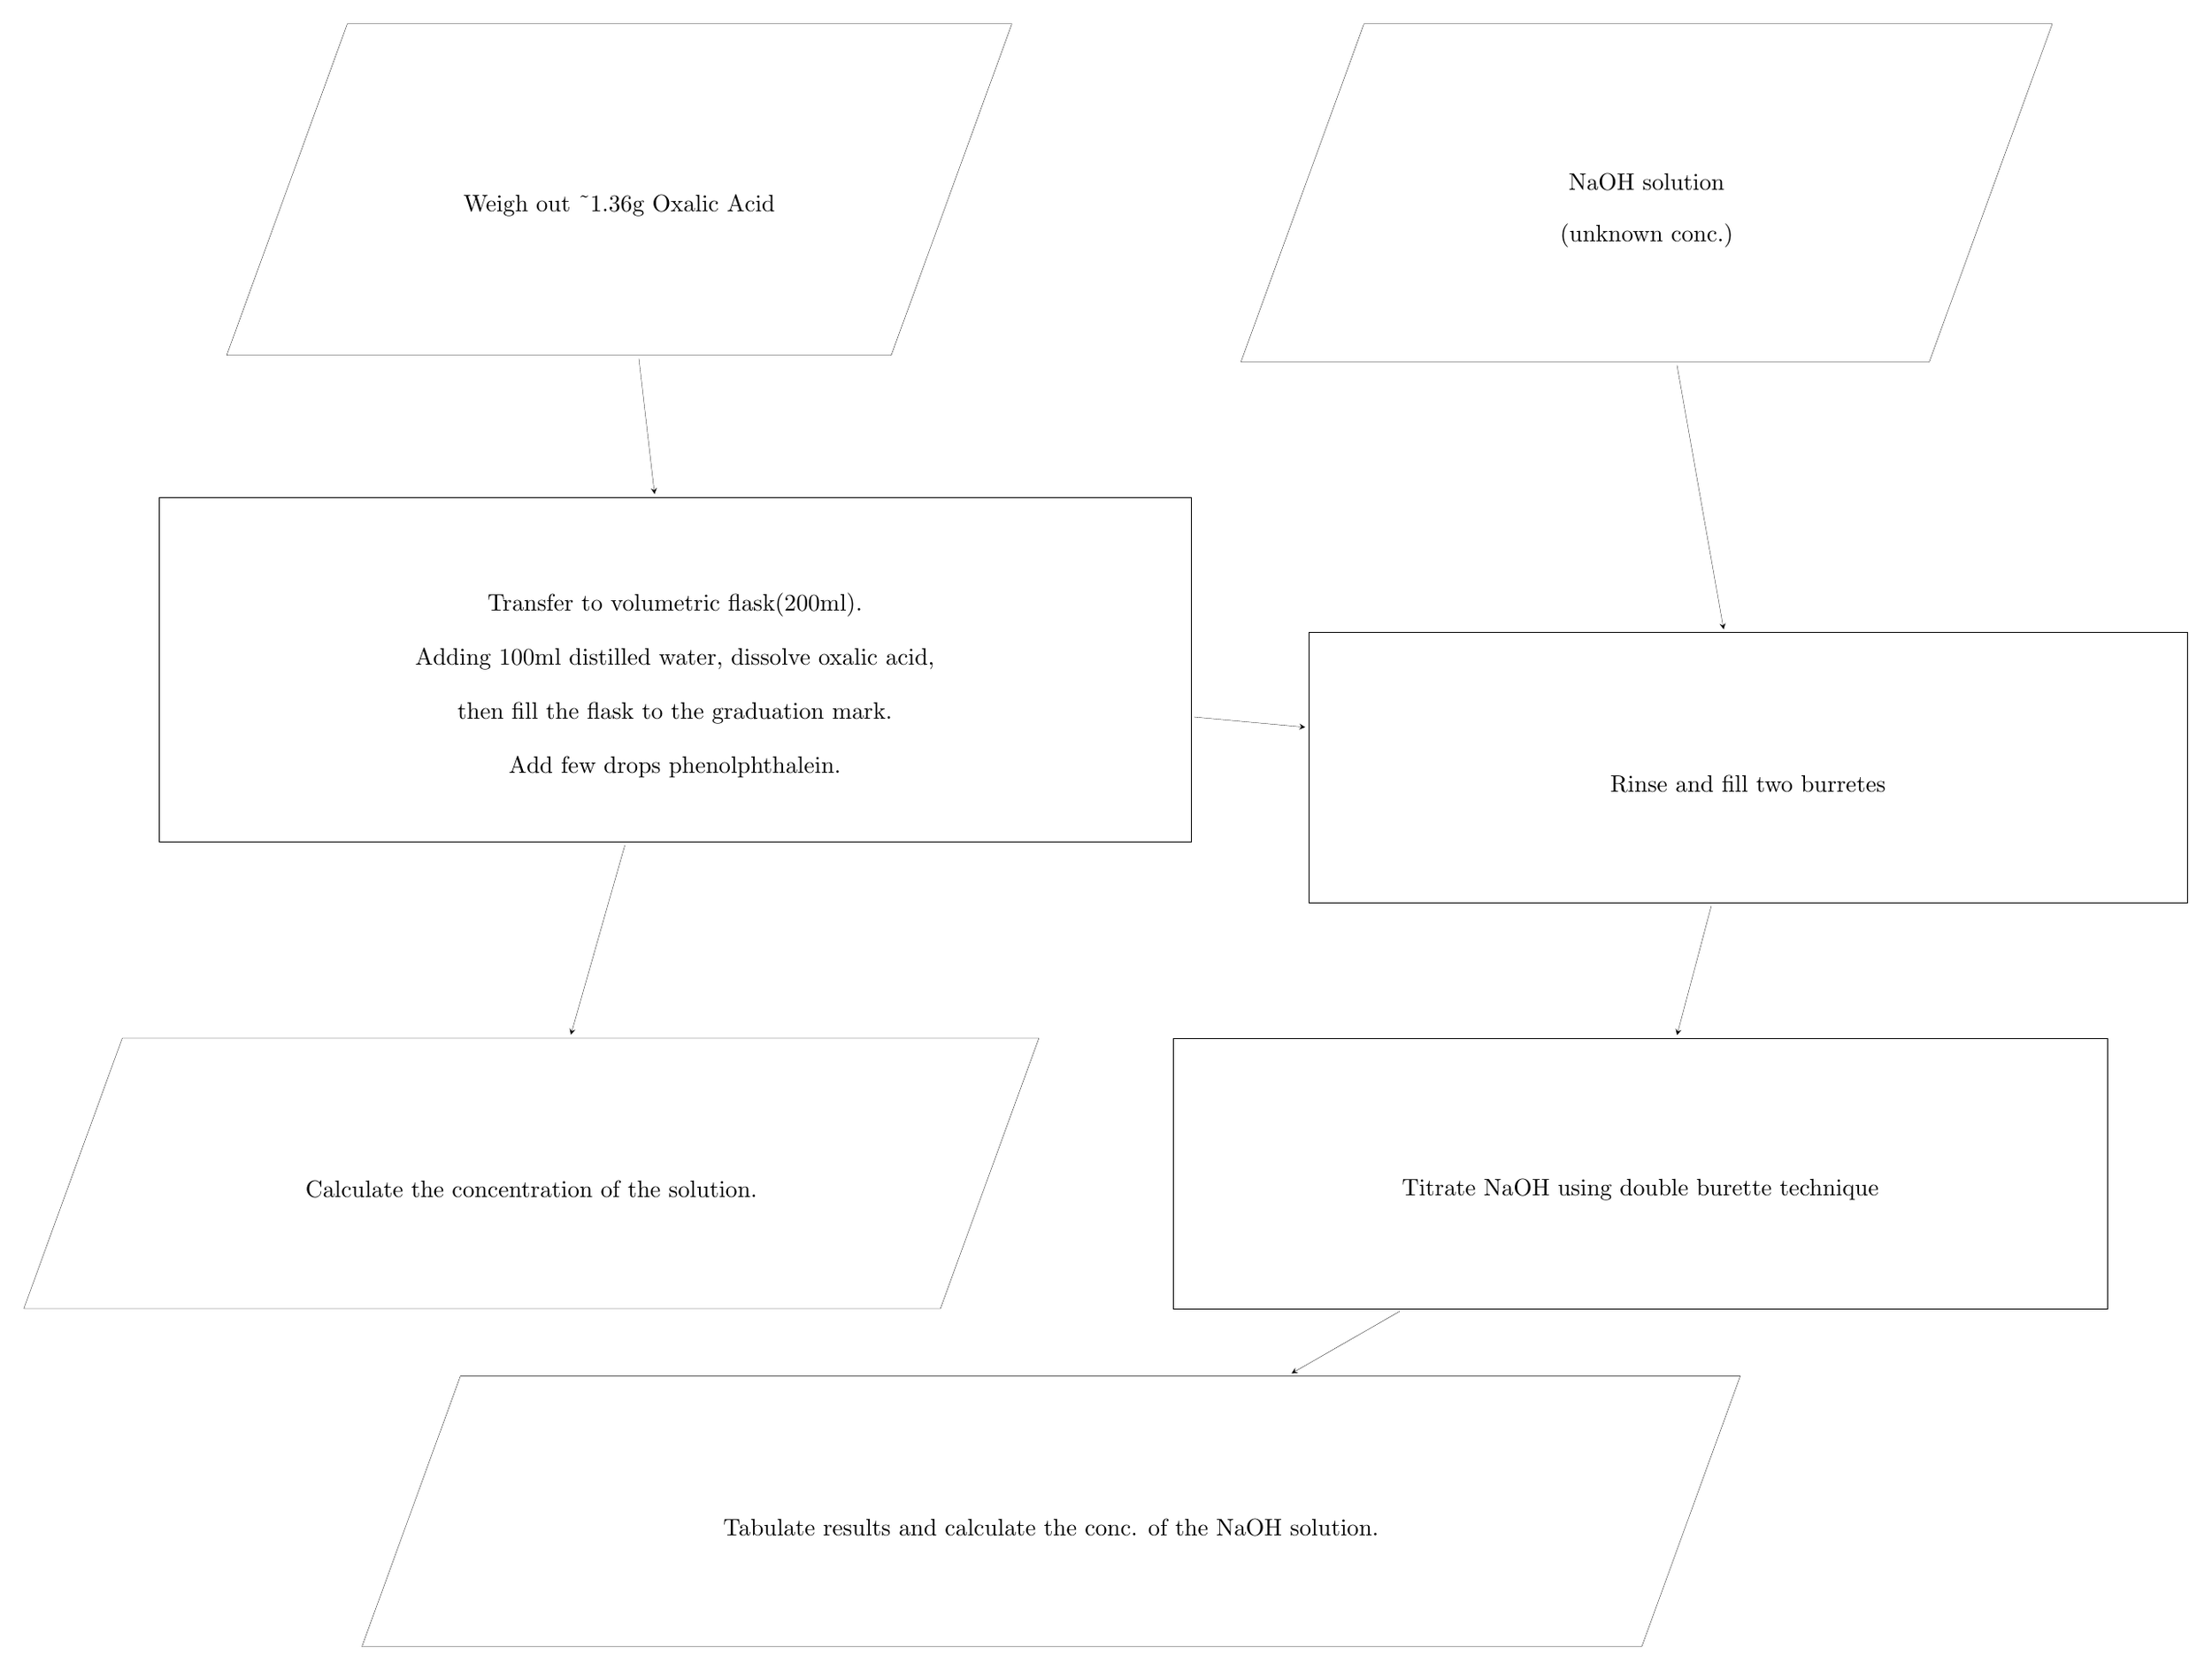
\begin{tikzpicture}
\pgftransformxscale{1.000000}
\pgftransformyscale{-1.000000}
\definecolor{dialinecolor}{rgb}{0.000000, 0.000000, 0.000000}
\pgfsetstrokecolor{dialinecolor}
\definecolor{dialinecolor}{rgb}{1.000000, 1.000000, 1.000000}
\pgfsetfillcolor{dialinecolor}
\definecolor{dialinecolor}{rgb}{1.000000, 1.000000, 1.000000}
\pgfsetfillcolor{dialinecolor}
\fill (-8.216546\du,0.000000\du)--(1.612130\du,0.000000\du)--(-0.171324\du,4.900000\du)--(-10.000000\du,4.900000\du)--cycle;
\pgfsetlinewidth{0.100000\du}
\pgfsetdash{}{0pt}
\pgfsetdash{}{0pt}
\pgfsetmiterjoin
\definecolor{dialinecolor}{rgb}{0.000000, 0.000000, 0.000000}
\pgfsetstrokecolor{dialinecolor}
\draw (-8.216546\du,0.000000\du)--(1.612130\du,0.000000\du)--(-0.171324\du,4.900000\du)--(-10.000000\du,4.900000\du)--cycle;
% setfont left to latex
\definecolor{dialinecolor}{rgb}{0.000000, 0.000000, 0.000000}
\pgfsetstrokecolor{dialinecolor}
\node at (-4.193935\du,2.690000\du){Weigh out \~{}1.36g Oxalic Acid};
\definecolor{dialinecolor}{rgb}{1.000000, 1.000000, 1.000000}
\pgfsetfillcolor{dialinecolor}
\fill (-11.000000\du,7.000000\du)--(-11.000000\du,12.100000\du)--(4.257500\du,12.100000\du)--(4.257500\du,7.000000\du)--cycle;
\pgfsetlinewidth{0.100000\du}
\pgfsetdash{}{0pt}
\pgfsetdash{}{0pt}
\pgfsetmiterjoin
\definecolor{dialinecolor}{rgb}{0.000000, 0.000000, 0.000000}
\pgfsetstrokecolor{dialinecolor}
\draw (-11.000000\du,7.000000\du)--(-11.000000\du,12.100000\du)--(4.257500\du,12.100000\du)--(4.257500\du,7.000000\du)--cycle;
% setfont left to latex
\definecolor{dialinecolor}{rgb}{0.000000, 0.000000, 0.000000}
\pgfsetstrokecolor{dialinecolor}
\node at (-3.371250\du,8.590000\du){Transfer to volumetric flask(200ml).};
% setfont left to latex
\definecolor{dialinecolor}{rgb}{0.000000, 0.000000, 0.000000}
\pgfsetstrokecolor{dialinecolor}
\node at (-3.371250\du,9.390000\du){ Adding 100ml distilled water, dissolve oxalic acid,};
% setfont left to latex
\definecolor{dialinecolor}{rgb}{0.000000, 0.000000, 0.000000}
\pgfsetstrokecolor{dialinecolor}
\node at (-3.371250\du,10.190000\du){then fill the flask to the graduation mark.};
% setfont left to latex
\definecolor{dialinecolor}{rgb}{0.000000, 0.000000, 0.000000}
\pgfsetstrokecolor{dialinecolor}
\node at (-3.371250\du,10.990000\du){Add few drops phenolphthalein.};
\pgfsetlinewidth{0.100000\du}
\pgfsetdash{}{0pt}
\pgfsetdash{}{0pt}
\pgfsetbuttcap
{
\definecolor{dialinecolor}{rgb}{0.000000, 0.000000, 0.000000}
\pgfsetfillcolor{dialinecolor}
% was here!!!
\pgfsetarrowsend{stealth}
\definecolor{dialinecolor}{rgb}{0.000000, 0.000000, 0.000000}
\pgfsetstrokecolor{dialinecolor}
\draw (-3.904258\du,4.949994\du)--(-3.672124\du,6.953369\du);
}
\definecolor{dialinecolor}{rgb}{1.000000, 1.000000, 1.000000}
\pgfsetfillcolor{dialinecolor}
\fill (-11.544119\du,15.000000\du)--(2.012057\du,15.000000\du)--(0.556176\du,19.000000\du)--(-13.000000\du,19.000000\du)--cycle;
\pgfsetlinewidth{0.100000\du}
\pgfsetdash{}{0pt}
\pgfsetdash{}{0pt}
\pgfsetmiterjoin
\definecolor{dialinecolor}{rgb}{0.000000, 0.000000, 0.000000}
\pgfsetstrokecolor{dialinecolor}
\draw (-11.544119\du,15.000000\du)--(2.012057\du,15.000000\du)--(0.556176\du,19.000000\du)--(-13.000000\du,19.000000\du)--cycle;
% setfont left to latex
\definecolor{dialinecolor}{rgb}{0.000000, 0.000000, 0.000000}
\pgfsetstrokecolor{dialinecolor}
\node at (-5.493971\du,17.240000\du){Calculate the concentration of the solution.};
\pgfsetlinewidth{0.100000\du}
\pgfsetdash{}{0pt}
\pgfsetdash{}{0pt}
\pgfsetbuttcap
{
\definecolor{dialinecolor}{rgb}{0.000000, 0.000000, 0.000000}
\pgfsetfillcolor{dialinecolor}
% was here!!!
\pgfsetarrowsend{stealth}
\definecolor{dialinecolor}{rgb}{0.000000, 0.000000, 0.000000}
\pgfsetstrokecolor{dialinecolor}
\draw (-4.111819\du,12.149133\du)--(-4.909783\du,14.949704\du);
}
\definecolor{dialinecolor}{rgb}{1.000000, 1.000000, 1.000000}
\pgfsetfillcolor{dialinecolor}
\fill (6.000000\du,9.000000\du)--(6.000000\du,13.000000\du)--(19.000000\du,13.000000\du)--(19.000000\du,9.000000\du)--cycle;
\pgfsetlinewidth{0.100000\du}
\pgfsetdash{}{0pt}
\pgfsetdash{}{0pt}
\pgfsetmiterjoin
\definecolor{dialinecolor}{rgb}{0.000000, 0.000000, 0.000000}
\pgfsetstrokecolor{dialinecolor}
\draw (6.000000\du,9.000000\du)--(6.000000\du,13.000000\du)--(19.000000\du,13.000000\du)--(19.000000\du,9.000000\du)--cycle;
% setfont left to latex
\definecolor{dialinecolor}{rgb}{0.000000, 0.000000, 0.000000}
\pgfsetstrokecolor{dialinecolor}
\node at (12.500000\du,11.240000\du){Rinse and fill two burretes};
\definecolor{dialinecolor}{rgb}{1.000000, 1.000000, 1.000000}
\pgfsetfillcolor{dialinecolor}
\fill (6.819851\du,0.000000\du)--(17.000000\du,0.000000\du)--(15.180149\du,5.000000\du)--(5.000000\du,5.000000\du)--cycle;
\pgfsetlinewidth{0.100000\du}
\pgfsetdash{}{0pt}
\pgfsetdash{}{0pt}
\pgfsetmiterjoin
\definecolor{dialinecolor}{rgb}{0.000000, 0.000000, 0.000000}
\pgfsetstrokecolor{dialinecolor}
\draw (6.819851\du,0.000000\du)--(17.000000\du,0.000000\du)--(15.180149\du,5.000000\du)--(5.000000\du,5.000000\du)--cycle;
% setfont left to latex
\definecolor{dialinecolor}{rgb}{0.000000, 0.000000, 0.000000}
\pgfsetstrokecolor{dialinecolor}
\node at (11.000000\du,2.340000\du){NaOH solution};
% setfont left to latex
\definecolor{dialinecolor}{rgb}{0.000000, 0.000000, 0.000000}
\pgfsetstrokecolor{dialinecolor}
\node at (11.000000\du,3.140000\du){(unknown conc.)};
\pgfsetlinewidth{0.100000\du}
\pgfsetdash{}{0pt}
\pgfsetdash{}{0pt}
\pgfsetbuttcap
{
\definecolor{dialinecolor}{rgb}{0.000000, 0.000000, 0.000000}
\pgfsetfillcolor{dialinecolor}
% was here!!!
\pgfsetarrowsend{stealth}
\definecolor{dialinecolor}{rgb}{0.000000, 0.000000, 0.000000}
\pgfsetstrokecolor{dialinecolor}
\draw (4.307184\du,10.251503\du)--(5.950591\du,10.401645\du);
}
\pgfsetlinewidth{0.100000\du}
\pgfsetdash{}{0pt}
\pgfsetdash{}{0pt}
\pgfsetbuttcap
{
\definecolor{dialinecolor}{rgb}{0.000000, 0.000000, 0.000000}
\pgfsetfillcolor{dialinecolor}
% was here!!!
\pgfsetarrowsend{stealth}
\definecolor{dialinecolor}{rgb}{0.000000, 0.000000, 0.000000}
\pgfsetstrokecolor{dialinecolor}
\draw (11.449890\du,5.049377\du)--(12.138916\du,8.953857\du);
}
\definecolor{dialinecolor}{rgb}{1.000000, 1.000000, 1.000000}
\pgfsetfillcolor{dialinecolor}
\fill (4.000000\du,15.000000\du)--(4.000000\du,19.000000\du)--(17.812500\du,19.000000\du)--(17.812500\du,15.000000\du)--cycle;
\pgfsetlinewidth{0.100000\du}
\pgfsetdash{}{0pt}
\pgfsetdash{}{0pt}
\pgfsetmiterjoin
\definecolor{dialinecolor}{rgb}{0.000000, 0.000000, 0.000000}
\pgfsetstrokecolor{dialinecolor}
\draw (4.000000\du,15.000000\du)--(4.000000\du,19.000000\du)--(17.812500\du,19.000000\du)--(17.812500\du,15.000000\du)--cycle;
% setfont left to latex
\definecolor{dialinecolor}{rgb}{0.000000, 0.000000, 0.000000}
\pgfsetstrokecolor{dialinecolor}
\node at (10.906250\du,17.240000\du){Titrate NaOH using double burette technique};
\definecolor{dialinecolor}{rgb}{1.000000, 1.000000, 1.000000}
\pgfsetfillcolor{dialinecolor}
\fill (-6.544119\du,20.000000\du)--(12.384557\du,20.000000\du)--(10.928676\du,24.000000\du)--(-8.000000\du,24.000000\du)--cycle;
\pgfsetlinewidth{0.100000\du}
\pgfsetdash{}{0pt}
\pgfsetdash{}{0pt}
\pgfsetmiterjoin
\definecolor{dialinecolor}{rgb}{0.000000, 0.000000, 0.000000}
\pgfsetstrokecolor{dialinecolor}
\draw (-6.544119\du,20.000000\du)--(12.384557\du,20.000000\du)--(10.928676\du,24.000000\du)--(-8.000000\du,24.000000\du)--cycle;
% setfont left to latex
\definecolor{dialinecolor}{rgb}{0.000000, 0.000000, 0.000000}
\pgfsetstrokecolor{dialinecolor}
\node at (2.192279\du,22.240000\du){Tabulate results and calculate the conc. of the NaOH solution.};
\pgfsetlinewidth{0.100000\du}
\pgfsetdash{}{0pt}
\pgfsetdash{}{0pt}
\pgfsetbuttcap
{
\definecolor{dialinecolor}{rgb}{0.000000, 0.000000, 0.000000}
\pgfsetfillcolor{dialinecolor}
% was here!!!
\pgfsetarrowsend{stealth}
\definecolor{dialinecolor}{rgb}{0.000000, 0.000000, 0.000000}
\pgfsetstrokecolor{dialinecolor}
\draw (11.956818\du,13.044922\du)--(11.449432\du,14.955078\du);
}
\pgfsetlinewidth{0.100000\du}
\pgfsetdash{}{0pt}
\pgfsetdash{}{0pt}
\pgfsetbuttcap
{
\definecolor{dialinecolor}{rgb}{0.000000, 0.000000, 0.000000}
\pgfsetfillcolor{dialinecolor}
% was here!!!
\pgfsetarrowsend{stealth}
\definecolor{dialinecolor}{rgb}{0.000000, 0.000000, 0.000000}
\pgfsetstrokecolor{dialinecolor}
\draw (7.349180\du,19.041016\du)--(5.749349\du,19.958984\du);
}
\end{tikzpicture}

        \end{adjustbox}
    \end{center}

    \subsubsection*{NaOH}
    \begin{itemize}
        \item Corrosive
        \item[-] avoid contact with skin and eyes
        \item[-] wash immediately if contact occurs
      \end{itemize}

      \subsubsection*{Oxalic Acid}
      \begin{itemize}
          \item Corrosive
          \item Harmful
          \item[-] avoid contact with skin and eyes, do not ingest.
          \item[-] wash immediately if contact occurs
        \end{itemize}

    \newpage

    \section{Pre-Practical Questions}

  pH values for questions 1 through 5 are shown in \cref{table:titration}. \Cref{fig:curve} is a plot of these vales to produce a titration curve.

    \begin{table}[htb]
        \centering
        \caption{Titration}
        \begin{tabular}{cc}
            \addlinespace
            \toprule
            HCl (ml) & pH \\ 
            \midrule
            0 & 10.972 \\
            10 & 9.421 \\
            12.5 & 9.245 \\
            25 & 5.361 \\
            26 & 2.881 \\ 
            \bottomrule
            \end{tabular}
            \label{table:titration}   
    \end{table}

    \begin{figure}[htb]
        \centering
        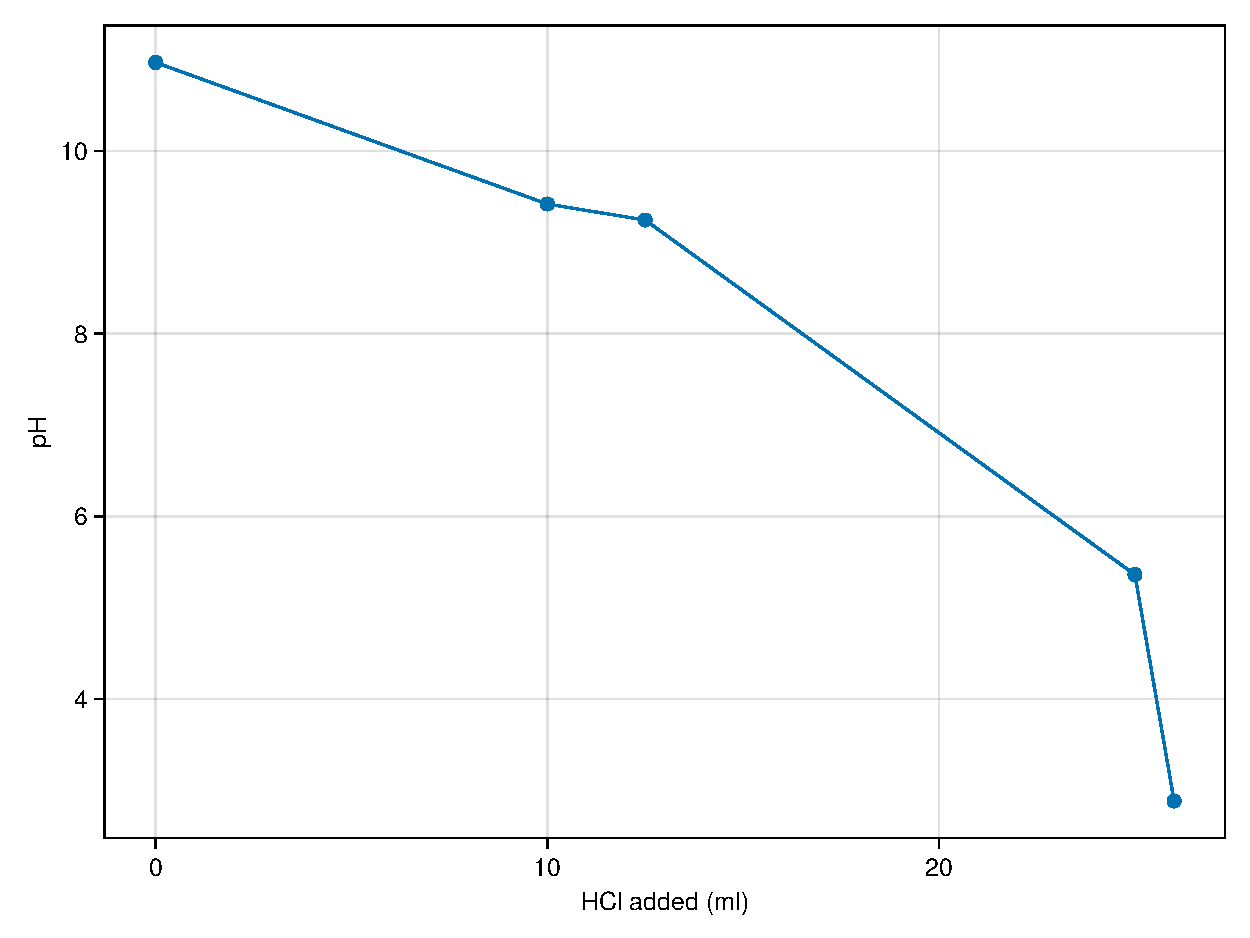
\includegraphics[width=\textwidth]{figures/curve.pdf}
        \caption{Titration Curve}
        \label{fig:curve}
    \end{figure}
    
\end{appendices}

\end{document}